%Resume penggunaan aplikasi testis webservice
%judul jurnal hari ke 1  IMPLEMENTASI REST WEB SERVICE UNTUK SALES ORDER DAN SALES TRACKING BERBASIS MOBILE
%judul jurnal hari ke 2  Penerapan Teknologi Web Service Untuk Integrasi Layanan Puskesmas dan Rumah Sakit
%Kelompok 5 D4 TI - 2B
%Fransiscus Ivan Martongam      1164039
%Lalita Chandiany Adiputri      1164043
%Eko Cahyono Putro              1164035
%Lidwina Triniska Gulo          1164044
%Sulpadianti Bunyamin           1164096


\section{Pengenalan WebService}
Web Services dengan arsitektur REST digunakan oleh berbagai macam jenis client seperti mobile, Web, dan Desktop.
Dapat membantu perusahaan untuk melakukan pelacakan, tracking terhadap tenaga penjual yang ditugaskan untuk menawarkan 
barang atau penagihan ke pelanggan. Dengan REST Web Services yang akan dibuat perusahaan akan dapat memastikan
bahwa semua tenaga penjual akan mengunjungi pelanggan sesuai dengan target yang sudah ditentukan oleh perusahaan.


\section{Arsitektur Web Services}
Architektur Web Service memiliki tiga komponen utama diantaranya yaitu Service provider adalah Penyedia web service yang berfungsi
menyediakan kumpulan web services yang dapat diaksesoleh pengguna.Service requesto adalah aplikasi yang bertindak sebagai pengguna yang
melakukan permintaan layanan (berupaweb services) keservice provider.Service registry adalah tempat dimana service provider 
mempublikasikan layanannya. Pada arsitekturWeb service,Service registry bersifat opsional.

\ref{arsitektur}
\centerline{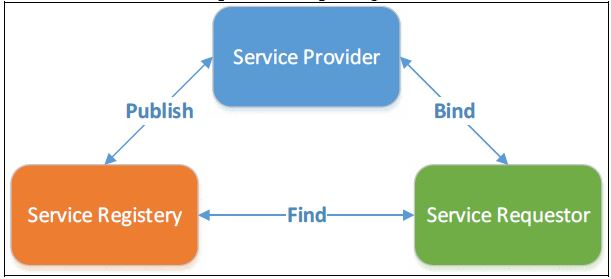
\includegraphics[width=1\textwidth]{figures/arsitektur.PNG}}
\caption{arsitektur web service}
\lable{arsitektur}
\end{figure}


\section{rest dalam penggunaan testing web service}
REST adalah filosofi desain yang mendorong untuk menggunakan protokol dan fitur yang sudah ada pada Web. Pada web services akan dapat memaksimalkan kinerja web services terutama pada performa, skalabilitas, dan kemudahan untuk dimodifikasi. Bentuk web service menggunakan REST style digunakan sebagai backend dari aplikasi berbasis mobile karena cara aksesnya  mudah dan hasil data yang dikirimkan berformat JSON sehingga ukuran file menjadi lebih kecil. 


\section{web api}
Web API adalah antar muka program dari sistem yang dapat diakses lewat method dan
header pada protokol HTTP yang standar. Web API dapat diakses dari berbagai macam HTTP
client seperti browser dan perangkat mobile. Web API juga memiliki keuntungan karena
menggunakan infrastruktur yang juga digunakan oleh web terutama untuk penggunaan caching
dan concurrency.


\section{Perancangan Sistem}
Aplikasi yang akan dibuat terdiri dari dua bagian besar yaitu aplikasi yang ada pada bagian client dan bagian server. Aplikasi yang ada di server bertugas menyediakan data yang dapat digunakan oleh aplikasi client, aplikasi client digunakan untuk meminta data dari aplikasi yang ada di server. Web services dipilih dengan beberapa pertimbangan yaitu agar memudahkanpembangunan proses bisnis yang dapat digunakan untuk berbagai macam client tanpa harus membuat proses tersebut secara spesifik berdasarkan teknologi client yang digunakan.


\section{Implementasi Web service Berbasis ASP.NET}
Dalam proses pembuatan Web Services berbasis ASP.NET terdapat beberapa services atau fungsi-fungsi yang dibuat untuk mengakses database SQL Server. Services-services tersebut yang nantinya dipanggil dan digunakan untuk membangun sistem integrasi layanan puskesmasdan rumah sakit berbasis Web Services.Proses integrasi sistem dengan Web Services berbasis asp dapat dilakukan dengan penggunaan dokumen WSDL yang dapat diakses pada alamat WSDL-nya http://192.168.1.100:8080/wsrs/Service.asmx?WSDL dan hasil dari skema WSDLnya.
